\begin{figure}[H]
    \centering
    \tikzset{every picture/.style={line width=0.75pt}} %set default line width to 0.75pt        
    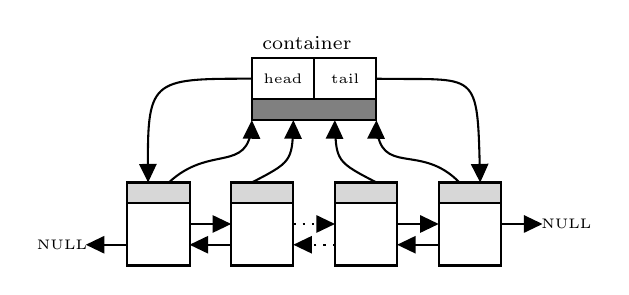
\begin{tikzpicture}[x=0.75pt,y=0.75pt,yscale=-1,xscale=1]
        \foreach \x in {250,300,350,400}{ %draw left arrows
           \draw [shift={(\x,130)}, rotate = 180] [fill=black ][line width=0.08]  [draw opacity=0] (8.93,-4.29) -- (0,0) -- (8.93,4.29) -- cycle ;
        }
        \foreach \x in {180,230,280,330}{ %draw right arrow
           \draw [shift={(\x,140)}, rotate = 360] [fill=black ][line width=0.08]  [draw opacity=0] (8.93,-4.29) -- (0,0) -- (8.93,4.29) -- cycle ;
        }
        %draw down arrows
        \draw [shift={(370,110)}, rotate = 268.47] [fill=black][line width=0.08] [draw opacity=0] (8.93,-4.29) -- (0,0) -- (8.93,4.29) -- cycle;
        \draw [shift={(210,110)}, rotate = 269.43] [fill=black][line width=0.08] [draw opacity=0] (8.93,-4.29) -- (0,0) -- (8.93,4.29) -- cycle;
        
        \foreach \x in {260,280,300,320}{ %draw up arrows
            \draw [shift={(\x,80)}, rotate = 451.07] [fill=black ][line width=0.08]  [draw opacity=0] (8.93,-4.29) -- (0,0) -- (8.93,4.29) -- cycle ;
        }
        %draw arrow connections
        \draw    (200,140) -- (183,140) ;
        \draw    (250,140) -- (233,140) ;
        \draw    (350,140) -- (333,140) ;
        \draw  [dash pattern={on 0.84pt off 2.51pt}]  (300,140) -- (283,140) ;
        \draw    (330,130) -- (347,130) ;
        \draw    (380,130) -- (397,130) ;
        \draw    (230,130) -- (247,130) ;
        \draw  [dash pattern={on 0.84pt off 2.51pt}]  (280,130) -- (297,130) ;
    
        \draw  [fill=gray ,fill opacity=1 ] (260,70) -- (320,70) -- (320,80) -- (260,80) -- cycle ;
        \foreach \x in {200,250,300,350}{%draw list nodes
            \draw  [fill=lightgray  ,fill opacity=0.62 ] (\x,110) -- (\x+30,110) -- (\x+30,120) -- (\x,120) -- cycle ;  
            \draw   (\x,110) -- (\x+30,110) -- (\x+30,150) -- (\x,150) -- cycle ;
        }
        \draw   (260,50) -- (290,50) -- (290,70) -- (260,70) -- cycle ;
        \draw   (290,50) -- (320,50) -- (320,70) -- (290,70) -- cycle ;
        %draw up and down arrow connections
        \draw    (320,60) .. controls (369.74,60.99) and (368.55,54.07) .. (369.93,107.52) ;
        \draw    (260,60) .. controls (210.51,60) and (209.52,60) .. (209.97,107.06) ;
        \draw    (220,110) .. controls (239.78,91.53) and (258.17,105.78) .. (259.88,82.67) ;
        \draw    (260,110) .. controls (278.52,100.36) and (279.45,99.88) .. (279.93,82.83) ;
        \draw    (320,110) .. controls (301.47,100.36) and (300.55,99.88) .. (300.07,82.83) ;
        \draw    (360,110) .. controls (341.18,90.56) and (321.9,107.58) .. (320.12,82.86) ;
        %draw tags
        \draw (275,60) node  [font=\tiny] [align=left] {\lstinline{head}};
        \draw (305,60) node  [font=\tiny] [align=left] {\lstinline{tail}};
        \draw (286.5,43) node  [font=\scriptsize] [align=left] {container};
        \draw (168.5,140) node  [font=\tiny] [align=left] {\lstinline{NULL}};
        \draw (411.5,130) node  [font=\tiny] [align=left] {\lstinline{NULL}};
    \end{tikzpicture}
    \caption{Doubly-linked list implementation}
    \label{fig:qlistsfigure}
\end{figure}